The first challenge I faced while designing the project was finding the best yet cheapest hardware to power the system efficiently, ensuring it could handle the required tasks without exceeding budget constraints, while also providing flexibility and scalability for future upgrades.

\begin{figure}[h]
    \centering
    \begin{minipage}[b]{0.32\textwidth}
        \centering
        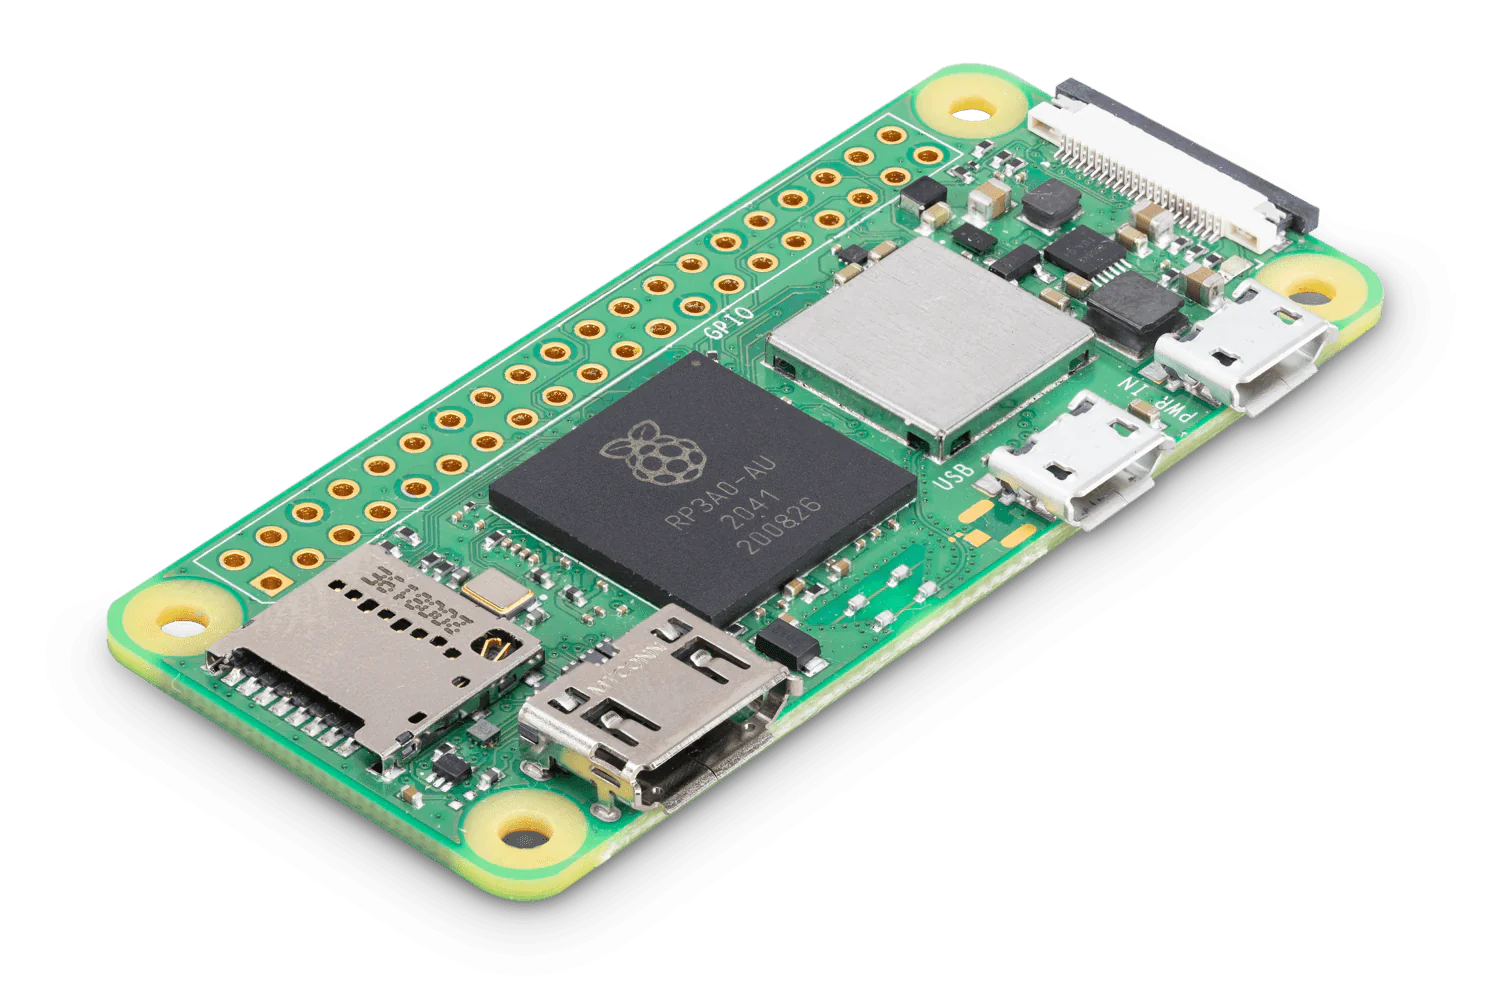
\includegraphics[width=\textwidth]{tesi/img/hardware_components/rpi.png}
        \caption*{Raspberry Pi Zero W}
    \end{minipage}
    \begin{minipage}[b]{0.32\textwidth}
        \centering
        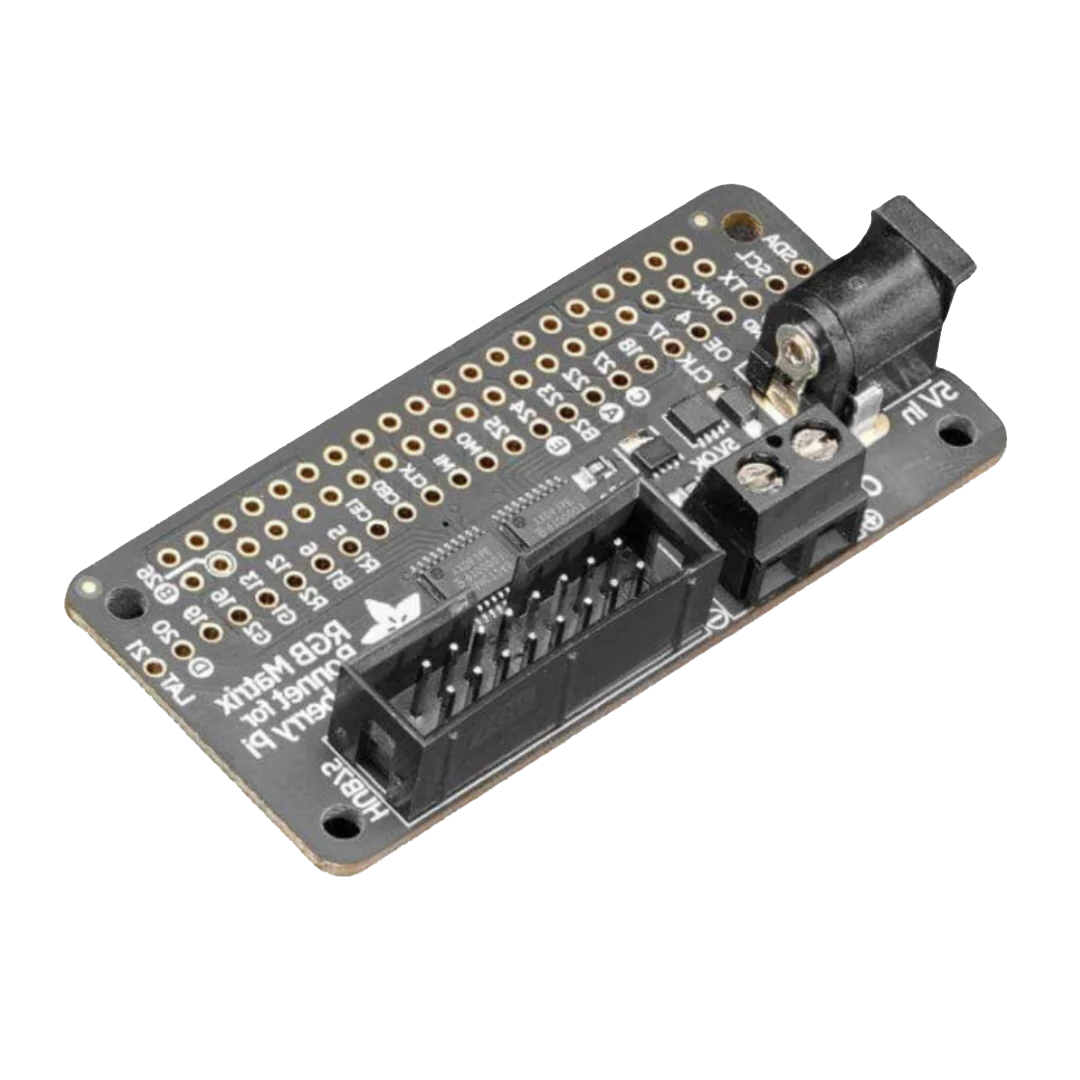
\includegraphics[width=\textwidth]{tesi/img/hardware_components/bonnet.png}
        \caption*{Adafruit RGB Matrix Bonnet}
    \end{minipage}
    \begin{minipage}[b]{0.32\textwidth}
        \centering
        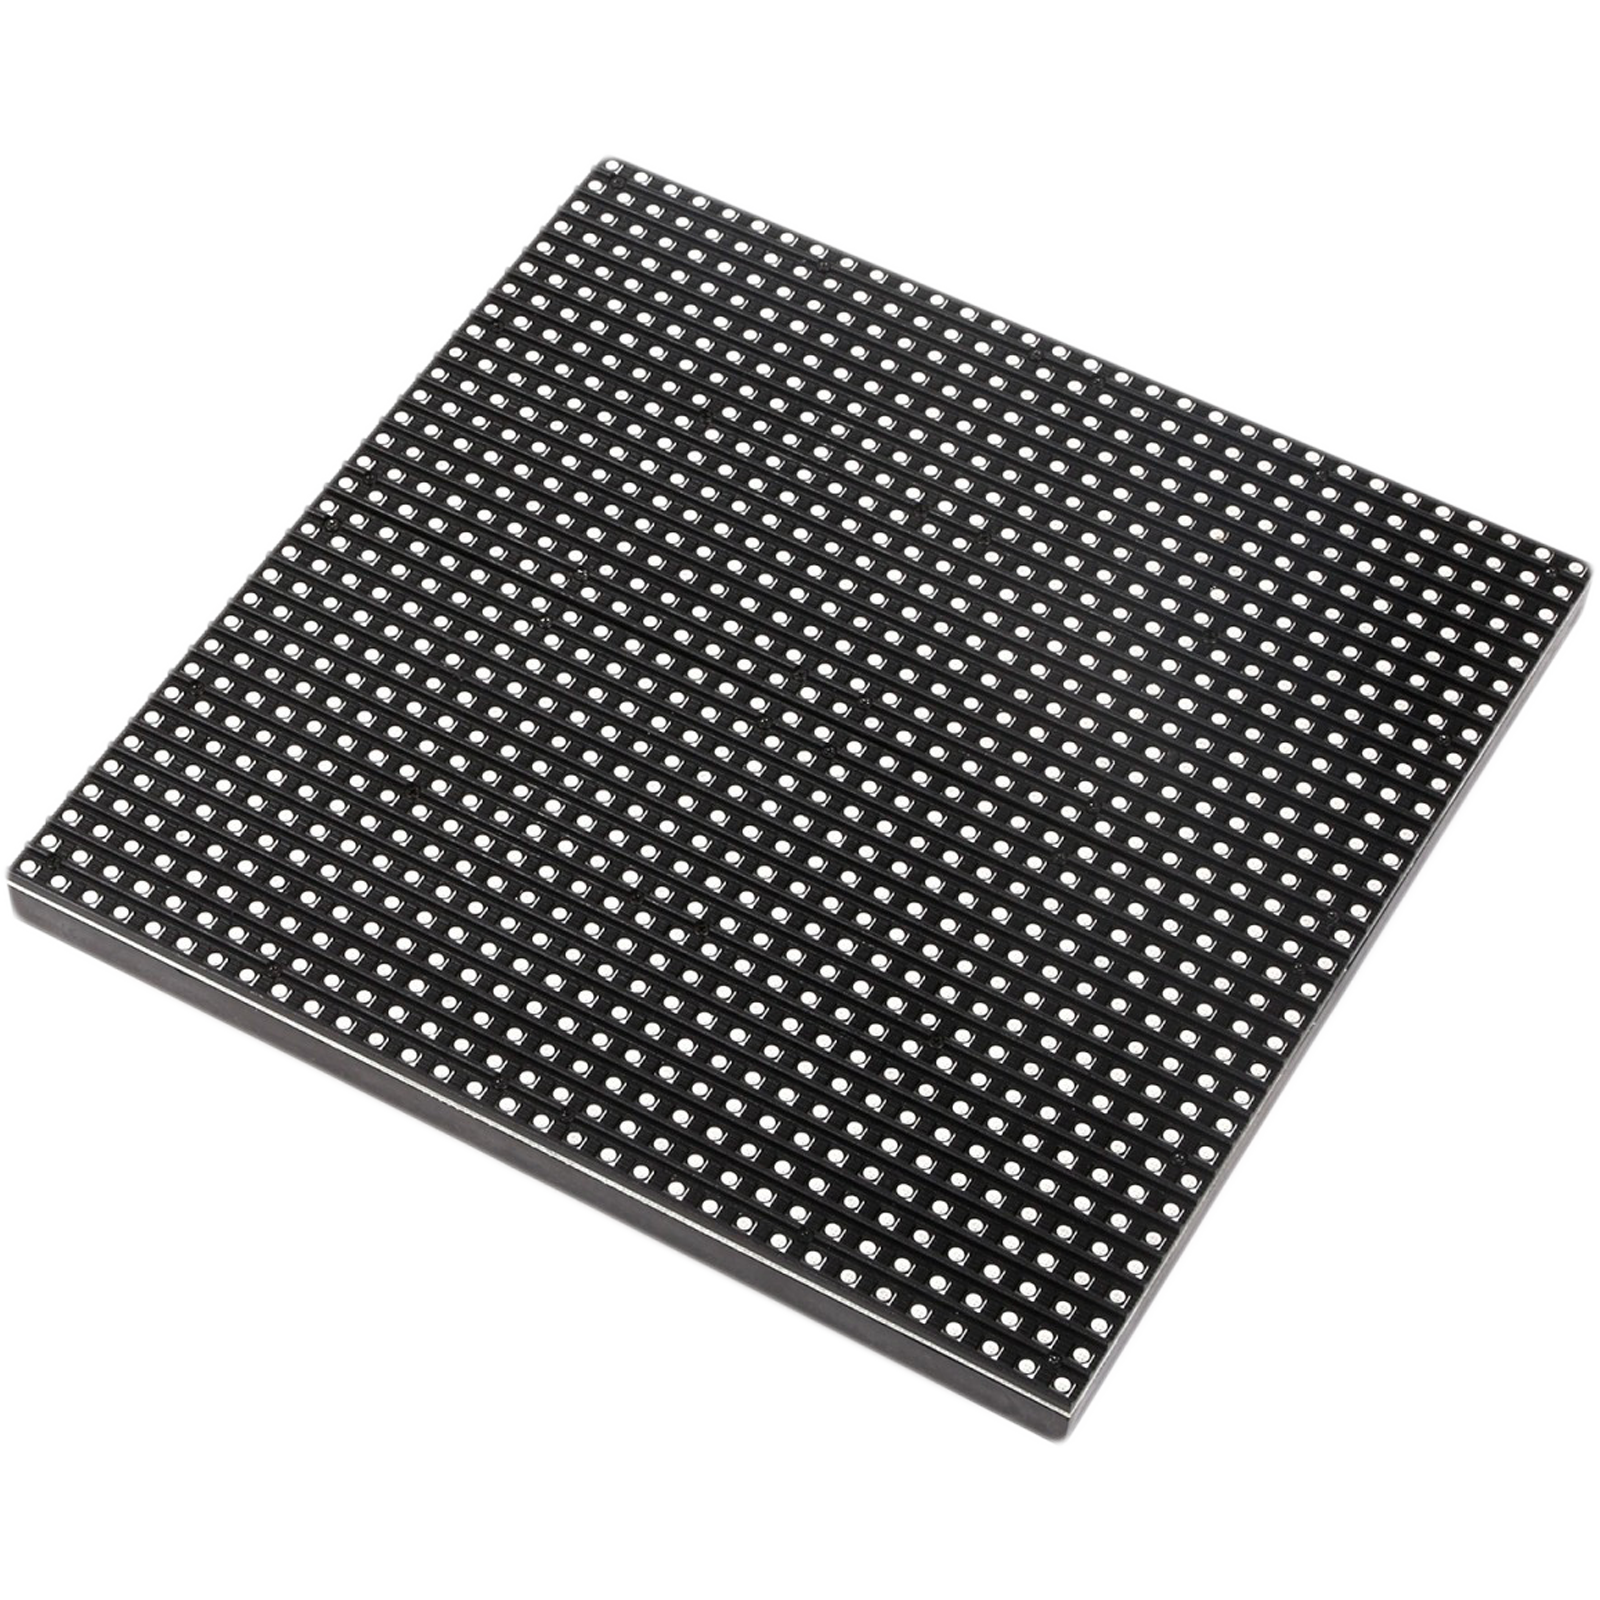
\includegraphics[width=\textwidth]{tesi/img/hardware_components/matrix.png}
        \caption*{Standard 64x64 LED Matrix}
    \end{minipage}
\end{figure}


\section{The SBC}

The most critical decision was selecting the processing unit,
and I realized that I needed a single-board computer (SBC) with the following
characteristics:

\begin{itemize}
	\item Sufficient computational power for handling both graphical rendering and networking operations

	\item Broad connectivity options, such as WiFi, Bluetooth, and GPIO pins for
		external peripherals

	\item Cost-effective, as affordability was a primary concern

	\item Highly customizable, to allow flexible development and integration with
		other components
\end{itemize}

Initially, I considered two options: the \textbf{Raspberry Pi} and the \textbf{ESP32}, both
equipped with built-in Bluetooth and WiFi. The ESP32 is a fantastic microcontroller, known for its low power consumption and versatility in IoT applications. It's gaining immense popularity due to its ultra-low cost—priced as low as 5 euros—yet powerful enough to build impressive and innovative projects.
However,
after evaluating my project’s requirements, I opted for the Raspberry Pi Zero W due
to its Linux support, which I believed would provide better flexibility and
facilitate more advanced functionalities, such as running a full operating system,
handling networking tasks, and interacting with various software libraries.

I chose the Raspberry Pi Zero W for several reasons:
\begin{itemize}
	\item \textbf{Operating System Support:} With a lightweight, CLI only Linux-based OS like \href{https://dietpi.com/}{DietPi}, I could leverage a vast ecosystem of software tools and libraries,
		enabling more complex operations that would be harder to achieve on a
		microcontroller like the ESP32.

	\item \textbf{Connectivity:} The Raspberry Pi Zero W comes with built-in WiFi
		and Bluetooth, making it ideal for connecting to the internet and integrating
		with other wireless devices.

	\item \textbf{Size and Power Consumption:} Despite being a fully capable
		computer, the Raspberry Pi Zero W is compact and consumes minimal power,
		which was important for keeping the hardware cost-effective and portable.

	\item \textbf{GPIO Pins:} The GPIO pins offer a wide range of possibilities
		for connecting sensors, LEDs, and other hardware components, making it easy to
		extend the platform with additional functionality.
\end{itemize}
\section{The Matrix}
When it came to selecting the LED matrix, I was faced with a wide array of options, each offering different resolutions, sizes, brands, and even color configurations. The first decision I had to make was regarding the resolution, which would directly impact the amount of information the display could render. The two primary options I considered were a rectangular 64x32 matrix or a square 64x64 matrix. After careful consideration, I ultimately chose the 64x64 matrix. This resolution struck the perfect balance for my needs: it wasn't too large, which kept the overall system compact and cost-effective, yet it provided enough screen real estate to display a substantial amount of information, ensuring that the display would be both functional and visually appealing.
\section{The Matrix Bonnet}
Although it would have been possible to manually wire the Raspberry Pi directly to the LED matrix, I decided to invest in the Matrix Bonnet for several reasons. For just a few euros, the bonnet offered a much safer, more reliable, and easier solution compared to manual wiring. It not only simplifies the connection process but also reduces the risk of damaging the components due to incorrect wiring. The Matrix Bonnet is specifically designed for use with Raspberry Pi boards, allowing for seamless integration and a cleaner, more stable setup. It handles all the necessary data and power connections without the hassle of complex wiring, which saved me significant time and effort during development. The bonnet is just one of the many incredible products developed by Adafruit Industries, which are designed to make open-source DIY projects like this not only accessible but also well-documented and enjoyable\footnote{\url{https://www.adafruit.com}}.

\section{Future Upgrades}
While the current setup meets the initial goals of the project, I have plans for several future upgrades to enhance both functionality and user experience. I am considering integrating new sensor types, such as environmental sensors or cameras, to add real-time data collection capabilities. 